\begin{figure}
\begin{center}

% 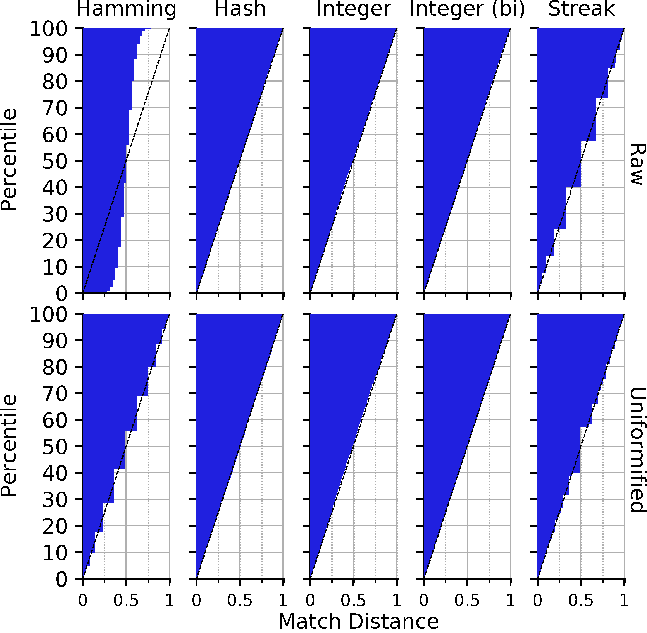
\includegraphics[width=\columnwidth]{img/uniformification/bitweight=0dot5+seed=1+title=low-score-distribution+_data_hathash_hash=75684cf1e73fb7f1+_script_fullcat_hash=c3113c80efb02374+ext=}
\begin{minipage}{\linewidth}
\begin{subfigure}[b]{\linewidth}
\begin{minipage}{0.75\textwidth}
\begin{center}
\includegraphics[width=\columnwidth]{img/uniformification/bitweight=0dot5+seed=1+title=low-score-distribution+viz=hist+_data_hathash_hash=75684cf1e73fb7f1+_script_fullcat_hash=2f100d81b8ad6826+ext=}
\end{center}
\end{minipage}
\begin{minipage}{0.23\textwidth}
\caption{
Histogram visualization of match distance between randomly sampled tags.
The bin count of 64 was chosen to emphasize the coarse match distance discretization imposed by the Streak metric and the Hamming metric.
Error bars are 95\% confidence intervals calculated using the Wilson score method with continuity correction \citep{newcombe1998two}.
}
\label{fig:uniformification_hist}
\end{minipage}
\end{subfigure}
\end{minipage}

\begin{minipage}{\linewidth}
\begin{subfigure}[b]{\linewidth}
\begin{minipage}{0.75\textwidth}
\begin{center}
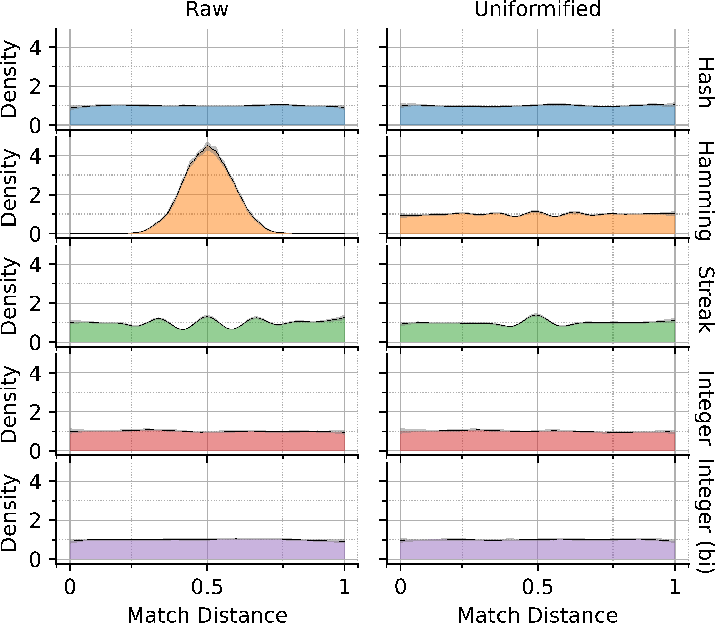
\includegraphics[width=\columnwidth]{img/uniformification/bitweight=0dot5+seed=1+title=low-score-distribution+viz=kde+_data_hathash_hash=75684cf1e73fb7f1+_script_fullcat_hash=73c1663bd9b49595+ext=}
\end{center}
\end{minipage}
\begin{minipage}{0.23\textwidth}
\caption{
Kernel density estimate visualization of match distance between randomly sampled tags.
Estimated density incorporates linear combination correction for bounded distributions due to restriction of match distance within the interval $[0,1]$ \citep{jones1993simple}.
Gray error bands are bootstrap 95\% confidence intervals over 1,000 resamplings.
}
\label{fig:uniformification_kde}
\end{minipage}
\end{subfigure}
\end{minipage}

\caption{
Distance distributions of metrics before and after uniformification.
A sample of 5,000 distances between randomly-generated tag pairs was used for each plot.
Subfigure \ref{fig:uniformification_hist} emphasizes the discretization artifacts in the Hamming and Streak metrics present before and remaining after uniformification.
(E.g., for 32-bit tags under the Hamming metric only 32 distinguishable match distance values are possible.)
Subfigure \ref{fig:uniformification_kde} masks distribution discretization to more intuitively depict the corrected metrics' approximation of a uniform distribution.
}
\label{fig:uniformification}

\end{center}
\end{figure}
